% !TEX root = benchmark_tables_standalone.tex
%
% ── PENDIENTES ─────────────────────────────────────────────────────
%
% --- Análisis por hacer ---
% TODO 1: Para las μ no detectadas (ej. QPCBLEND 63/67), revisar cuál
%         de los 4 criterios falla en cada una. Esto dice cuál criterio
%         es el cuello de botella.
% TODO 2: Examinar la estructura de F — ¿por qué κ apenas mejora en
%         QPCBLEND? (1.77e11 → 1.69e11). Puede explicar TODO 3.
% TODO 3: ¿Por qué QPCBLEND no mejora mucho con K̂? (56% eliminación,
%         conectado a estructura de F y a TODO 1).
%
% --- Justificaciones por escribir ---
% TODO 4: Justificar por qué 5 iteraciones adicionales con K̂.
%         (Tabla 7 ya lo muestra: iter 1 no mejora, 2-4 hacen el trabajo,
%         5+ se estanca. Escribir el argumento en el texto.)
% TODO 5: Justificar por qué eliminar-y-después-iterar en vez de
%         eliminar gradualmente. (La detección necesita el historial
%         completo de la fase con K para estabilizarse.)
%
% --- Redacción ---
% TODO 6: Arreglar "eliminados" en sección Condicionamiento.
% TODO 7: Criterio z*/μ* > 100: mencionar que se eligió empíricamente.
% TODO 8: Revisar umbral de Tapia (0.8 puede no ser óptimo).
%
% ───────────────────────────────────────────────────────────────────
%
% ====================================================================
% Informe de avance — Resultados benchmark (heurística de eliminación)
% ====================================================================
\newcommand{\hldig}[1]{{\setlength{\fboxsep}{0.5pt}\colorbox{yellow!40}{$#1$}}}
\newcommand{\nuevo}[1]{\textcolor{blue}{#1}}
% Marcas de referencias pendientes al unir con main.tex. Borrar macro y usos al limpiar.
\newcommand{\falta}[1]{{\color{red}\footnotesize\textsf{[FALTA: #1]}}}

\section*{WHAT WE WILL DO NEXT? HAHA}\label{sec:experimentos}

En esta sección describiremos la estrategia computacional para la heurística propuesta al final del \hyperref[subsec:heuristica]{capítulo anterior}. La metodología será la siguiente:
\begin{enumerate}
    \item Primero compararemos la precisión de nuestros resultados del IPM contra un solver independiente (Clarabel) y contra los valores publicados en la literatura, usando 9~problemas provenientes de dos fuentes: Maros \& Meszaros (MM)\footnote{Maros, I.\ y Meszaros, C.\ (1999). ``A Repository of Convex Quadratic Programming Problems''. \textit{Optim.\ Methods Softw.}, 11(1--4), 671--681. \href{https://doi.org/10.1080/10556789908805768}{DOI: 10.1080/10556789908805768}. Archivos \texttt{.mat}: \href{https://github.com/YimingYAN/QP-Test-Problems}{github.com/YimingYAN/QP-Test-Problems}.} y Hock \& Schittkowski (HS) \footnote{Hock, W.\ y Schittkowski, K.\ (1981). \textit{Test Examples for Nonlinear Programming Codes}. Lecture Notes in Economics and Mathematical Systems, vol.~187, Springer. \href{https://doi.org/10.1007/978-3-642-48320-2}{DOI: 10.1007/978-3-642-48320-2}.} (Tabla~\ref{tab:benchmark_problems}).
\falta{estas dos notas al pie deben ser \texttt{\textbackslash cite\{marosmeszaros1999\}} y \texttt{\textbackslash cite\{hock1981\}}; ambas ya están en bibliography.bib}
    \item Con la solución de Clarabel, identificaremos cuáles $\mu_i$ tienden realmente a cero; esta será nuestra referencia.
    \item Aplicaremos los cinco criterios durante el IPM y veremos si las restricciones que marca el método coinciden con las de Clarabel.
    \item Eliminaremos esas filas y columnas para obtener un sistema reducido $\widehat{K}$ con mejor condicionamiento.
    \item Usaremos $\widehat{K}$ para continuar iterando y compararemos la solución con la que se obtiene al seguir iterando con~$K$.
    \item Aplicaremos el método a algunos problemas de dimensiones mayores y compararemos contra el trabajo de Montiel\falta{\texttt{\textbackslash cite\{MontielGonzalez2023\}}}, contrastando con el uso de precondicionadores.
    \item Por último, analizaremos cómo afecta cada criterio a nuestros resultados y a la eliminación de restricciones.
\end{enumerate}
Los experimentos se ejecutan en un MacBook Pro con procesador Intel Core i5-6360U a 2.0\,GHz, 8\,GB de RAM, macOS~12.7, Python~3.14, NumPy~2.4 y SciPy~1.17. La aritmética es de punto flotante IEEE~754 de doble precisión ($\varepsilon_{\text{mach}} \approx 2.2 \times 10^{-16}$).

\bigskip

% ---------------------------------------------------------------------------
% NO SE IMPRIME. "Recordatorio del problema": repite \eqref{P1} y el sistema K de
% main.tex. Al unir, sustituir por referencias en vez de reescribirlos.
%
% \subsection*{Recordatorio del problema}
% \falta{al unir: este recordatorio repite \eqref{P1} y el sistema $K$ de main.tex. Sustituir por referencias a \texttt{P1} y \texttt{eq:KKT\_reduced} en vez de reescribirlos, o dejarlo muy abreviado}
%
% Nuestro problema tiene la estructura
% \begin{equation}
% \begin{aligned}
% \min_{x \in \mathbb{R}^n}\quad & \frac{1}{2}\,x^T Q x + c^T x \\
% \text{s.a.}\quad & Ax - b = \mathbf{0}_m, \\
% \quad & Fx - d \ge \mathbf{0}_p \\
% \end{aligned}
% \tag{P1}
% \end{equation}
% donde $f(x) = \tfrac{1}{2} x^T Q x + c^T x$, $g(x)=Fx-d$ y $h(x)=Ax-b$, y adicionalmente tiene las siguientes características:
% \[
% \begin{aligned}
% & Q \in \mathbb{R}^{n \times n}, \text{ simétrica y } Q \text{ es definida positiva, i.e. }  Q \succ 0, \quad c \in \mathbb{R}^{n}, \\[1mm]
% & A \in \mathbb{R}^{m \times n}, \ \operatorname{rank}(A) = m, \quad b \in \mathbb{R}^{m}, \ m \le n, \\[1mm]
% & F \in \mathbb{R}^{p \times n}, \quad d \in \mathbb{R}^{p}
% \end{aligned}
% \]
%
% \medskip
%
% Las holguras son $z = Fx - d \in \mathbb{R}^p$ ($z \ge \mathbf{0}_p$), los multiplicadores $\lambda\in\mathbb{R}^m$ para igualdad y $\mu\in\mathbb{R}^p$ ($\mu\ge\mathbf{0}_p$) para desigualdad. Complementariedad: $\mu_j z_j = 0$ para todo $j$.
%
% \medskip
%
% Con $D_\mu = \operatorname{diag}(\mu)$, $D_z = \operatorname{diag}(z)$, y el cambio de variable $D_\mu^{-1}\delta_\mu$, el sistema reducido ($n+m+p$) que resolvemos cada iteración es:
%
% \begin{equation}
% \underbrace{
% \begin{pmatrix}
% Q & -A^T & -F^T D_\mu \\
% -A & \mathbf{0}_{m \times m} & \mathbf{0}_{m \times p} \\
% - D_\mu F & \mathbf{0}_{p \times m} & - D_z D_\mu
% \end{pmatrix}}_K
% \begin{pmatrix}
% \delta_x \\[1mm]
% \delta_\lambda \\[1mm]
% D_\mu^{-1} \delta_\mu
% \end{pmatrix}
% =
% -
% \underbrace{
% \begin{pmatrix}
% Qx + c - A^T \lambda - F^T \mu \\[1mm]
% - Ax + b \\[1mm]
% D_\mu(d - Fx) + \tau e
% \end{pmatrix}}_L
% \tag{K}
% \end{equation}
%
% Para resolver el sistema $K\delta = -L$ en cada iteración se utiliza \texttt{scipy.linalg.solve}, que maneja de forma robusta sistemas cercanos a la singularidad emitiendo un aviso cuando el condicionamiento es alto.
% \falta{enlazar con el párrafo de main.tex donde se explica que usamos un método directo y no iterativo, a diferencia de Montiel}
% ---------------------------------------------------------------------------

% =====================================================================
\section*{Problemas de prueba}
% =====================================================================

Los valores de referencia de los problemas HS son analíticos (del libro); los de MM son los que reportan los autores (obtenidos con el solver BPMPD\footnote{BPMPD: solver de punto interior para programación lineal y cuadrática desarrollado por Meszaros (1999).}\falta{usar \texttt{\textbackslash cite\{Meszaros1999bpmpd\}}}).
Los valores publicados de MM no tienen más dígitos de precisión que lo reportado a continuación.

% TABLE 1
\begin{table}[H]
\centering
\caption{Problemas de prueba y valores de referencia.}
\label{tab:benchmark_problems}
\begin{tabular}{lrrr r l}
\toprule
Problema & $n$ & $m$ & $p$ & $f^*$ publicado & Fuente \\
\midrule
TAME     &   2 &  1 &   2 &  $0$             & MM \\
HS21     &   2 &  0 &   5 & $-99.96$        & HS \\
HS35     &   3 &  0 &   4 &  $\frac{1}{9}$          & HS \\[3pt]
HS53     &   5 &  3 &  10 &  $\frac{176}{43}$       & HS \\
DUAL1    &  85 &  1 & 170 &  $0.03501297$   & MM \\
DUAL2    &  96 &  1 & 192 &  $0.03373368$   & MM \\
DUAL3    & 111 &  1 & 222 &  $0.13575584$   & MM \\
DUAL4    &  75 &  1 & 150 &  $0.74609084$   & MM \\
QPCBLEND &  83 & 43 & 114 & $-0.00784254$   & MM \\
\bottomrule
\end{tabular}
\end{table}


% =====================================================================
\section*{Metodología}
% =====================================================================

\subsection*{Paso 1: Verificación contra un solver independiente}

%Desafortunadamente, los resultados de referencia no incluyen los valores del vector $\mu$; lo cual quisiéramos utilizar para comparar con los resultados de nuestro IPM.
%Sin embargo, podemos aprovechar utilizar un solver independiente que nos arroje para obtener datos tales como la holgura $z^*$ y el multiplicador dual $\mu^*$.
%Al final, estamos diciendo que lo que estamos buscando averiguar es cuáles $\mu_i$ realmente tienden a cero, a partir de los resultados de un solver independiente.

El solver independiente escogido para este objetivo fue Clarabel\footnote{Goulart, P.\,J.\ y Chen, Y.\ (2024). ``Clarabel: An Interior-Point Solver for Conic Programs with Quadratic Objectives''. \href{https://arxiv.org/abs/2405.12762}{arXiv:2405.12762}.}.
\falta{usar \texttt{\textbackslash cite\{GoulartChen2024\}}}
Dicho solver se destaca por atacar los problemas de precisión numérica combinando una factorización $LDL^T$ (análoga a Cholesky, pero no requiere que la matriz sea definida positiva) y el esquema predictor-corrector de Mehrotra para resolver el sistema KKT de forma estable y acelerar su convergencia. Además, es de código abierto (\textit{open-source}) y es accesible desde Python a través de la librería \texttt{qpsolvers}.

Verificamos que la solución de Clarabel coincide con los valores publicados (Tabla~\ref{tab:clarabel_oracle}). Utilizando \texttt{solve\_problem} de \texttt{qpsolvers}, las diferencias son del orden de $10^{-9}$ o menos:

% TABLE 2a
\begin{table}[H]
\centering
\caption{Verificación: Clarabel vs valores publicados.}
\label{tab:clarabel_oracle}
\begin{tabular}{l r r r}
\toprule
Problema & $f^*$(Clarabel) & $f^*$(publicado) & $|\text{dif}|$ \\
\midrule
TAME     &  $0.0000000000$ &  $0.0000000000$ & $0$ \\
HS21     & $-99.9$\hldig{599999991} & $-99.9$\hldig{600000000} & $8.9\times10^{-10}$ \\
HS35     &  $0.11111111$\hldig{83} &  $0.11111111$\hldig{11} & $7.2\times10^{-9}$ \\
HS53     &  $4.0930232558$ &  $4.0930232558$ & $8.9\times10^{-16}$ \\
DUAL1    &  $0.03501296$\hldig{88} &  $0.03501296$\hldig{60} & $2.8\times10^{-9}$ \\
DUAL2    &  $0.033733676$\hldig{2} &  $0.033733676$\hldig{0} & $2.4\times10^{-10}$ \\
DUAL3    &  $0.1357558$\hldig{379} &  $0.1357558$\hldig{400} & $2.1\times10^{-9}$ \\
DUAL4    &  $0.74609084$\hldig{19} &  $0.74609084$\hldig{00} & $1.9\times10^{-9}$ \\
QPCBLEND & $-0.00784254$\hldig{20} & $-0.00784254$\hldig{09} & $1.1\times10^{-9}$ \\
\bottomrule
\end{tabular}

\vspace{0.3em}
\footnotesize
Los dígitos resaltados indican dónde $f^*$ diverge del valor publicado.
\end{table}

\subsection*{Paso 1b: Clasificación de referencia (Clarabel)}

La función \texttt{solve\_problem} nos proporciona la solución primal~$x^*$, los multiplicadores duales de desigualdad~$\mu^*$ y de igualdad~$\lambda^*$, además del valor objetivo reportado anteriormente~$f^*$.
Dicha función, desafortunadamente, no proporciona información sobre dichos valores durante las iteraciones del método, entonces sí debemos tomar en cuenta que el criterio para determinar que $\mu_i \to 0$ será algo arbitrario, pero con justificación.
Recordemos que, por la condición de complementariedad, al menos uno de los dos es cero en la solución óptima.
Cuando exactamente uno de los dos términos de la condición es cero, no solo se satisface la condición de complementariedad, sino que la complementariedad es estricta.

Para clasificar, usaremos el cociente $z_i^*/\mu_i^*$: si $z_i^*/\mu_i^* > 100$, la holgura domina y $\mu_i \to 0$ (restricción inactiva); si $z_i^*/\mu_i^* < \frac{1}{100}$, el dual domina y $z_i \to 0$ (restricción activa).
Para las restricciones con cociente entre $\frac{1}{100}$ y $100$, se considerarán demasiado ambiguas y no se eliminarán. La ventaja de utilizar el cociente es que compara $z_i^*$ y $\mu_i^*$ entre sí, en lugar de depender de un umbral absoluto sobre la magnitud de alguno de los dos.

Adelanto al lector que al examinar los cocientes $z_i^*/\mu_i^*$ de las 869~restricciones totales de los 9~problemas, se observará una separación natural que nos permite definir este criterio.
El cociente más alto debajo de 100 es $\approx 40$, mientras que el cociente más bajo por arriba de 100 es de magnitud $\approx 105$. En total, solo 7~restricciones de 869 son de magnitudes que consideramos demasiado ambiguas para decir con certeza que $\mu_i \to 0$.

La Figura~\ref{fig:ratio_separation} muestra los 869~cocientes ordenados de menor a mayor. La separación entre las restricciones activas ($z_i^*/\mu_i^* < \frac{1}{100}$) e inactivas ($z_i^*/\mu_i^* > 100$) es clara; la zona ambigua (sombreada) contiene solo 7~restricciones.

\begin{figure}[ht]
\centering
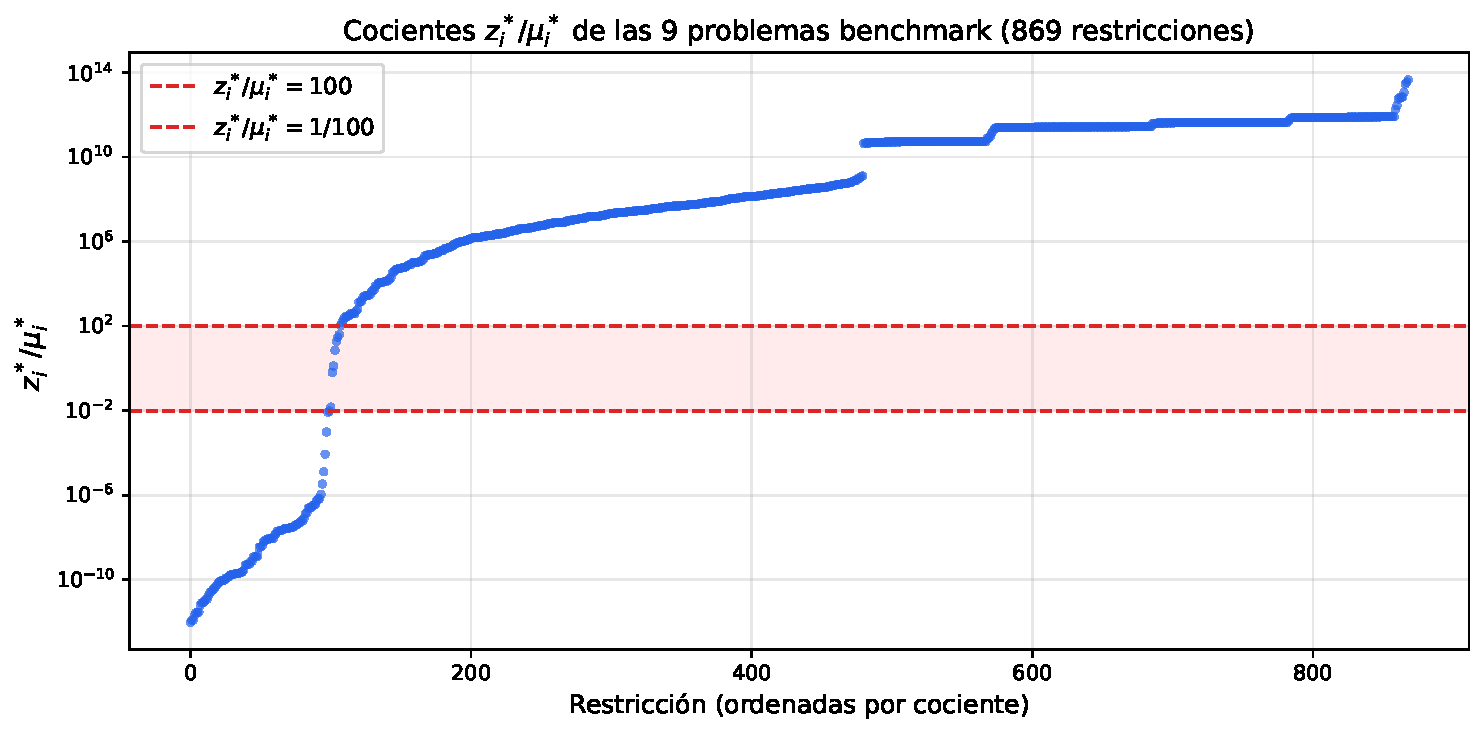
\includegraphics[width=0.85\textwidth]{ratio_separation.pdf}
\caption{Cocientes $z_i^*/\mu_i^*$ de las 869~restricciones de los 9~problemas, ordenados de menor a mayor. La zona sombreada ($\frac{1}{100} \le z_i^*/\mu_i^* \le 100$) contiene solo 7~restricciones.}
\label{fig:ratio_separation}
\end{figure}

% TABLE 2b
\begin{table}[H]
\centering
\caption{Clasificación de restricciones según el cociente $z_i^*/\mu_i^*$ (Clarabel).}
\label{tab:clarabel_classification}
\begin{tabular}{l r r r r}
\toprule
Problema & $p$ & $\mu_i\to0$ & $z_i\to0$ & \% $\mu_i\to0$ \\
\midrule
TAME     &   2 &   2 &   0 & 100\% \\
HS21     &   5 &   4 &   1 &  80\% \\
HS35     &   4 &   3 &   1 &  75\% \\
HS53     &  10 &  10 &   0 & 100\% \\
DUAL1    & 170 & 147 &  23 &  86\% \\
DUAL2    & 192 & 188 &   4 &  98\% \\
DUAL3    & 222 & 205 &  17 &  92\% \\
DUAL4    & 150 & 136 &  14 &  91\% \\
QPCBLEND & 114 &  67 &  47 &  59\% \\
\bottomrule
\end{tabular}

\vspace{0.3em}
\footnotesize
$\mu\to0$: restricciones con $z_i^*/\mu_i^* > 100$. \% del total = $\mu\to0$ / $p$.
\end{table}

% =====================================================================
\section*{Resultados}
% =====================================================================

Aplicamos los cinco criterios a los 9~problemas y evaluamos tres aspectos: si el método marca correctamente las restricciones con $\mu_i \to 0$, cómo cambia el condicionamiento de~$\widehat{K}$, y si las iteraciones adicionales con $\widehat{K}$ mejoran la solución. En estos 9~problemas usamos la tolerancia $\varepsilon_{\text{tol}} = 10^{-7}$.
Después repetimos el proceso con los problemas de NETLIB, que son de mayor dimensión, y al final analizamos más a fondo el papel de cada criterio en estos resultados.

\subsection*{Paso 2: Detección de $\mu_i \to 0$}

Utilizando los cinco criterios de la Tabla~\ref{tab:detection_criteria}, el método no marca ninguna restricción como $\mu_i \to 0$ cuando no lo es (0~errores en los 9~problemas, Tabla~\ref{tab:ipm_detection}).
QPCBLEND identifica el 75\% (50 de 67) porque el criterio $\mu_i < z_i$ descarta restricciones donde $\mu_i$ y $z_i$ son de magnitud similar y no es claro cuál tiende a cero.
Sin embargo, es preferible ser conservador a marcar una restricción de manera incorrecta.

% TABLE 3
\begin{table}[H]
\centering
\caption{Detección del IPM (5 criterios) vs clasificación de Clarabel.}
\label{tab:ipm_detection}
\begin{tabular}{l r r r r r r}
\toprule
         & & \multicolumn{1}{c}{Clarabel} & \multicolumn{3}{c}{Detección (IPM)} & \\
\cmidrule(lr){3-3} \cmidrule(lr){4-6}
Problema & Iter($K$) & $\mu_i\!\to\!0$ & Det. & \% & Err. & $\|x-x^*\|_\infty$ \\
\midrule
TAME     &  6 &   2 &   2 & 100\% & 0 & $1.1\times10^{-16}$ \\
HS21     & 11 &   4 &   4 & 100\% & 0 & $8.7\times10^{-8}$ \\
HS35     &  7 &   3 &   3 & 100\% & 0 & $5.6\times10^{-8}$ \\
HS53     &  8 &  10 &  10 & 100\% & 0 & $2.2\times10^{-11}$ \\
DUAL1    & 15 & 147 & 140 &  95\% & 0 & $3.8\times10^{-5}$ \\
DUAL2    & 13 & 188 & 185 &  98\% & 0 & $1.0\times10^{-5}$ \\
DUAL3    & 14 & 205 & 202 &  99\% & 0 & $2.5\times10^{-5}$ \\
DUAL4    & 12 & 136 & 136 & 100\% & 0 & $1.8\times10^{-5}$ \\
QPCBLEND & 22 &  67 &  50 &  75\% & 0 & $6.0\times10^{-5}$ \\
\bottomrule
\end{tabular}

\vspace{0.3em}
\footnotesize
\% Detección\ = Detectados / $\mu\to0$ real. Erróneas = restricciones detectadas como $\mu\to0$ que según Clarabel no lo son.
\end{table}


\subsection*{Paso 3: Condicionamiento de $\widehat{K}$}

En la Tabla~\ref{tab:conditioning} se muestran los números de condición de $K$ y $\widehat{K}$, en la primera y en la quinta iteración adicional.

% TABLE 4
\begin{table}[H]
\centering
\caption{Condicionamiento de $K$ vs $\widehat{K}$.}
\label{tab:conditioning}
\small
\begin{tabular}{l r r r r r}
\toprule
 & & \multicolumn{2}{c}{Iteración 1} & \multicolumn{2}{c}{Iteración 5} \\
\cmidrule(lr){3-4} \cmidrule(lr){5-6}
Problema & \% eliminación & $\kappa(K)$ & $\kappa(\widehat{K})$ & $\kappa(K)$ & $\kappa(\widehat{K})$ \\
\midrule
TAME       & 100\% & $2.56\times10^{9}$  & $5.00\times10^{0}$  & $2.56\times10^{17}$ & $5.00\times10^{0}$  \\
HS21       &  80\% & $3.50\times10^{8}$  & $7.50\times10^{1}$  & $3.41\times10^{16}$ & $7.50\times10^{1}$  \\
HS35       &  75\% & $3.29\times10^{9}$  & $7.81\times10^{1}$  & $2.84\times10^{17}$ & $7.81\times10^{1}$  \\
HS53       & 100\% & $2.49\times10^{9}$  & $1.28\times10^{2}$  & $2.49\times10^{17}$ & $1.28\times10^{2}$  \\
DUAL1$^*$  &  82\% & $2.73\times10^{13}$ & $1.33\times10^{12}$ & $1.16\times10^{19}$ & $2.16\times10^{18}$ \\
DUAL2$^*$  &  96\% & $2.86\times10^{14}$ & $8.68\times10^{11}$ & $2.11\times10^{21}$ & $4.20\times10^{19}$ \\
DUAL3$^*$  &  91\% & $7.51\times10^{13}$ & $1.43\times10^{12}$ & $4.76\times10^{18}$ & $4.50\times10^{17}$ \\
DUAL4$^*$  &  91\% & $6.42\times10^{15}$ & $1.27\times10^{10}$ & $2.07\times10^{19}$ & $1.71\times10^{15}$ \\
QPCBLEND   &  44\% & $1.77\times10^{11}$ & $1.77\times10^{11}$ & $8.43\times10^{15}$ & $8.12\times10^{15}$ \\
\bottomrule
\end{tabular}

\vspace{0.3em}
\scriptsize
Iteración $j$: matriz que se resuelve en la $j$-ésima iteración adicional; la iteración~1 corresponde al punto de convergencia.\\
$^*$\,$\sigma_{\min}(K) < \varepsilon\,\sigma_{\max}(K)$: el número de condición puede no ser confiable por cercanía a singularidad numérica.
\end{table}

Se observan tres comportamientos. En los problemas pequeños (TAME, HS21, HS35, HS53), la eliminación reduce $\widehat{K}$ a un sistema de dimensión muy baja (2--8) y $\kappa$ baja de $\sim\!10^{9}$ a $\sim\!10^{1}$--$10^{2}$.
En los problemas DUAL, la mejora es grande (por ejemplo DUAL4: de $10^{15}$ a $10^{10}$) pero $\kappa(\widehat{K})$ sigue siendo alto. A pesar de que cada fila de~$F$ tiene una sola entrada no nula (al igual que en los problemas pequeños), $Q$ es densa (${\sim}97\%$ de entradas no nulas) y domina el condicionamiento del sistema reducido, que aún tiene dimensión ${\sim}90$--$116$.
En QPCBLEND, $\kappa(\widehat{K}) = \kappa(K)$. A diferencia de los demás problemas, donde cada fila de~$F$ es $\pm e_j$ (una sola entrada no nula), QPCBLEND tiene filas de~$F$ con hasta 10~entradas no nulas y coeficientes de hasta ${\sim}66$, lo que acopla las variables. Al eliminar solo el 44\% de las restricciones, las 64~restantes siguen introduciendo esa dependencia y el condicionamiento no mejora.

\subsection*{Paso 4: Iteraciones adicionales con $\widehat{K}$}

Para comparar, también continuamos iterando con $K$ completo, a pesar de ya haber alcanzado la tolerancia indicada.
Es importante notar que los valores publicados de los problemas DUAL y QPCBLEND fueron obtenidos con un solver (BPMPD) y no son analíticos. Por lo tanto, la comparación de la precisión está limitada por el número de dígitos reportados en la referencia original.

Para aislar el efecto de la eliminación, se comparan $K$ y $\widehat{K}$ con exactamente 5~iteraciones adicionales después de la convergencia.
La Tabla~\ref{tab:f_K_vs_Khat} compara los valores de $f^*$ obtenidos con ambos sistemas, junto con la norma KKT que alcanza~$\widehat{K}$.

% TABLE 8 (merged: f* with highlighted digits + dimensions)
\begin{table}[H]
\centering
\caption{$f^*$ después de 5~iteraciones adicionales con $K$ vs $\widehat{K}$.}
\label{tab:f_K_vs_Khat}
\scriptsize
\begin{tabular}{l r r r r r r}
\toprule
Problema & $\dim(K)$ & $\dim(\widehat{K})$ & $f^*$(pub.) & $f^*$ ($K$, +5 iters) & $f^*$ ($\widehat{K}$, +5 iters) & $\|\text{KKT}\|_\infty$ ($\widehat{K}$, +5) \\
\midrule
TAME      &   5 &   3 & $0.0000000000$ & $0.0000000000$ & $0.0000000000$ & $0$ \\
HS21      &   7 &   3 & $-99.9600000000$ & $-99.9600000000$ & $-99.9600000000$ & $1.1\times10^{-17}$ \\
HS35      &   7 &   4 & $0.1111111111$ & $0.1111111111$ & $0.1111111111$ & $8.9\times10^{-16}$ \\
HS53      &  18 &   8 & $4.0930232558$ & $4.0930232558$ & $4.0930232558$ & $4.4\times10^{-16}$ \\
DUAL1$^*$ & 256 & 116 & $0.0350129660$ & $0.035012965\hldig{7}$ & $0.035012965\hldig{7}$ & $3.4\times10^{-14}$ \\
DUAL2$^*$ & 289 & 104 & $0.0337336760$ & $0.033733676\hldig{1}$ & $0.033733676\hldig{1}$ & $8.9\times10^{-16}$ \\
DUAL3$^*$ & 334 & 132 & $0.1357558400$ & $0.1357558\hldig{369}$ & $0.1357558\hldig{369}$ & $6.7\times10^{-11}$ \\
DUAL4$^*$ & 226 &  90 & $0.7460908400$ & $0.7460908\hldig{418}$ & $0.7460908\hldig{418}$ & $1.1\times10^{-14}$ \\
QPCBLEND  & 240 & 190 & $-0.0078425409$ & $-0.00784254\hldig{29}$ & $-0.00784254\hldig{29}$ & $1.4\times10^{-10}$ \\
\bottomrule
\end{tabular}

\vspace{0.3em}
\footnotesize
$^*$\,Valor publicado no analítico (obtenido con BPMPD).\\
Los dígitos resaltados indican dónde $f^*$ diverge del valor publicado.
\end{table}

Ambos sistemas alcanzan esencialmente la misma precisión. \nuevo{En todos los problemas los valores coinciden en todos los dígitos que reportamos (la mayor diferencia entre ambos es de $4\times10^{-12}$, en QPCBLEND), y la norma KKT con~$\widehat{K}$ es prácticamente la misma que con~$K$. Esto último no dice mucho sobre la precisión: al converger, los residuos $r_x$, $r_\lambda$ y $r_\mu$ ya están en precisión de máquina, así que la norma KKT mide sobre todo la complementariedad $\mu_i z_i$, que baja en cada iteración adicional. Lo que sí confirma es que al hacer $\mu_i = 0$ en las restricciones eliminadas no se pierde nada.}
Lo que empezamos a ver es que la ventaja de $\widehat{K}$ no es llegar a un mejor óptimo, sino llegar al mismo resolviendo un sistema más pequeño sin sacrificar precisión.
También hay que tomar en cuenta que las dimensiones de estos problemas son pequeñas: $\widehat{K}$ tiene a lo mucho dimensión ${\sim}190$. En problemas más grandes, donde el condicionamiento de~$K$ supera la precisión de máquina, la reducción de $\widehat{K}$ se vuelve no solo eficiente sino necesaria. Por eso, en el \hyperref[sec:netlib]{Paso~5} aplicamos el método a problemas \nuevo{más grandes: los mismos con los que trabajó Montiel.}

\subsection*{Paso 5: Problemas de NETLIB}
\label{sec:netlib}

Para ver qué pasa en problemas más grandes y peor condicionados, usamos los problemas de la colección NETLIB\footnote{Gay, D.\,M.\ (1985). ``Electronic mail distribution of linear programming test problems''. \textit{Mathematical Programming Society COAL Newsletter}, 13, 10--12. Archivos \texttt{.mat}: SuiteSparse Matrix Collection, grupo LPnetlib (Davis, T.\,A.\ y Hu, Y.\ (2011). ``The University of Florida Sparse Matrix Collection''. \textit{ACM Trans.\ Math.\ Softw.}, 38(1), 1:1--1:25), \href{https://sparse.tamu.edu/LPnetlib}{sparse.tamu.edu/LPnetlib}.}\falta{usar \texttt{\textbackslash cite\{Gay1985netlib\}} y \texttt{\textbackslash cite\{DavisHu2011\}}; ambas ya están en bibliography.bib} que utilizó Montiel\footnote{Montiel González, J.\ (2023). \textit{Precondicionadores en el método de puntos interiores para programación cuadrática convexa}. Tesis de Licenciatura en Matemáticas Aplicadas, ITAM.} en su tesis sobre precondicionadores para el IPM. Esto nos permite, además, comparar nuestro enfoque con el suyo.

Los problemas de NETLIB son de programación lineal. Siguiendo a Montiel, cada uno se convierte en un problema cuadrático de la forma
\[
\min_x\ x^Tx + c^Tx \quad \text{s.a.} \quad Ax = b, \quad x \ge 0,
\]
es decir, $Q = 2I$, $F = I$ y $d = 0$. Así, cada variable tiene su propia restricción de desigualdad y $p = n$. A diferencia de Montiel, quien toma $b = 0$, nosotros usamos el~$b$ original de cada problema: con $b = 0$, en muchos de ellos la solución es $x^* = 0$, todas las restricciones son activas y no hay ninguna $\mu_i \to 0$ que eliminar (véase el \hyperref[app:netlib_b0]{apéndice}). Usamos la misma tolerancia ($\|\text{KKT}\|_\infty < 10^{-6}$), el mismo máximo de 100~iteraciones y el mismo punto inicial (todas las variables en uno y $\lambda = 0$). De los 20~problemas de Montiel tenemos~18: no contamos con NESM ni SCSD8.

% TABLE NETLIB 1
\begin{table}[H]
\centering
\caption{Problemas de NETLIB: detección, condicionamiento y norma KKT con $K$ vs $\widehat{K}$.}
\label{tab:netlib}
\scriptsize
\setlength{\tabcolsep}{3pt}
\begin{tabular}{l r r r r r r r r r r}
\toprule
 & & & & & & \multicolumn{2}{c}{Iteración 1} & \multicolumn{2}{c}{Iteración 5} & \\
\cmidrule(lr){7-8} \cmidrule(lr){9-10}
Problema & $n$ & $m$ & Elim./$\mu\to0$ & \% & Err. & $\kappa(K)$ & $\kappa(\widehat{K})$ & $\kappa(K)$ & $\kappa(\widehat{K})$ & $\|\text{KKT}\|_\infty$ ($\widehat{K}$, +5) \\
\midrule
AFIRO & 51 & 27 & 39/42 & 93\% & 0 & $3.6\times10^{10}$ & $1.5\times10^{4}$ & $3.6\times10^{18}$ & $1.5\times10^{4}$ & $5.7\times10^{-14}$ \\
BLEND$^*$ & 114 & 74 & 82/86 & 95\% & 0 & $1.4\times10^{17}$ & $1.4\times10^{17}$ & $9.6\times10^{23}$ & $2.1\times10^{22}$ & $2.1\times10^{-13}$ \\
FIT1D$^*$ & 1049 & 24 & 303/309 & 98\% & 0 & $4.4\times10^{17}$ & $1.2\times10^{11}$ & $5.8\times10^{20}$ & $1.3\times10^{12}$ & $1.2\times10^{-10}$ \\
FIT1P$^*$ & 1677 & 627 & 833/843 & 99\% & 0 & $3.6\times10^{14}$ & $1.1\times10^{12}$ & $3.3\times10^{22}$ & $1.1\times10^{20}$ & $2.6\times10^{-10}$ \\
GROW7 & 301 & 140 & 205/216 & 95\% & 0 & $1.2\times10^{9}$ & $1.2\times10^{9}$ & $9.8\times10^{14}$ & $3.7\times10^{14}$ & $7.5\times10^{-10}$ \\
GROW15 & 645 & 300 & 476/500 & 95\% & 0 & $5.8\times10^{8}$ & $5.8\times10^{8}$ & $4.8\times10^{13}$ & $3.5\times10^{13}$ & $1.1\times10^{-13}$ \\
GROW22 & 946 & 440 & 689/752 & 92\% & 0 & $2.0\times10^{7}$ & $1.9\times10^{7}$ & $1.1\times10^{12}$ & $9.6\times10^{11}$ & $8.3\times10^{-10}$ \\
KB2 & 68 & 43 & 18/43 & 42\% & 0 & $5.3\times10^{10}$ & $5.3\times10^{10}$ & $6.1\times10^{15}$ & $6.9\times10^{15}$ & $4.0\times10^{-12}$ \\
RECIPE$^*$ & 204 & 91 & 89/141 & 63\% & 0 & $2.0\times10^{13}$ & $3.6\times10^{10}$ & $5.2\times10^{15}$ & $8.9\times10^{12}$ & $3.8\times10^{-10}$ \\
SCAGR7$^*$ & 185 & 129 & 0/172 & 0\% & 0 & $5.6\times10^{14}$ & --- & $5.6\times10^{22}$ & --- & $5.1\times10^{-12}$ \\
SCSD1 & 760 & 77 & 50/55 & 91\% & 0 & $8.9\times10^{11}$ & $5.3\times10^{11}$ & $5.0\times10^{16}$ & $4.6\times10^{16}$ & $5.8\times10^{-10}$ \\
SCSD6$^*$ & 1350 & 147 & 157/160 & 98\% & 0 & $2.2\times10^{13}$ & $2.2\times10^{13}$ & $1.3\times10^{17}$ & $1.1\times10^{17}$ & $3.1\times10^{-10}$ \\
SCTAP1$^*$ & 660 & 300 & 401/419 & 96\% & 0 & $2.8\times10^{19}$ & $3.3\times10^{19}$ & $2.5\times10^{23}$ & $5.0\times10^{22}$ & $1.5\times10^{-10}$ \\
SCTAP2$^*$ & 2500 & 1090 & 1570/1584 & 99\% & 0 & $7.9\times10^{15}$ & $7.9\times10^{15}$ & $6.8\times10^{29}$ & $2.5\times10^{27}$ & $6.0\times10^{-13}$ \\
SCTAP3$^*$ & 3340 & 1480 & 2177/2195 & 99\% & 0 & $1.8\times10^{16}$ & $1.8\times10^{16}$ & $6.4\times10^{21}$ & $3.2\times10^{24}$ & $2.1\times10^{-11}$ \\
SHARE2B$^*$ & 162 & 96 & 106/108 & 98\% & 0 & $2.0\times10^{14}$ & $4.7\times10^{10}$ & $3.8\times10^{21}$ & $4.7\times10^{18}$ & $5.2\times10^{-12}$ \\
STAIR$^*$ & 614 & 356 & 402/421 & 95\% & 0 & $2.4\times10^{18}$ & $2.4\times10^{18}$ & $4.5\times10^{28}$ & $1.1\times10^{27}$ & $9.1\times10^{-13}$ \\
STOCFOR1$^*$ & 165 & 117 & 110/110 & 100\% & 0 & $3.9\times10^{13}$ & $3.9\times10^{13}$ & $3.7\times10^{21}$ & $3.4\times10^{21}$ & $9.1\times10^{-13}$ \\
KLEEMINTY\_M3 & 6 & 3 & 0/5 & 0\% & 0 & $4.9\times10^{7}$ & --- & $4.6\times10^{15}$ & --- & $6.7\times10^{-16}$ \\
KLEEMINTY\_M5 & 10 & 5 & 8/8 & 100\% & 0 & $4.4\times10^{9}$ & $7.7\times10^{1}$ & $4.1\times10^{17}$ & $7.7\times10^{1}$ & $8.9\times10^{-16}$ \\
\bottomrule
\end{tabular}

\vspace{0.3em}
\footnotesize
$\mu\to0$: restricciones inactivas según Clarabel. $p = n$ en todos los problemas. ---: no se eliminó ninguna restricción, así que $\widehat{K} = K$.\\
Iteración $j$: matriz que se resuelve en la $j$-ésima iteración adicional; la iteración~1 corresponde al punto de convergencia.\\
$^*$\,$\sigma_{\min}(K) < \varepsilon\,\sigma_{\max}(K)$: el número de condición puede no ser confiable.
\end{table}

\nuevo{En los 20~problemas la heurística no marca ninguna restricción que no debería, y en casi todos identifica más del 90\% de las restricciones con $\mu_i \to 0$. Las excepciones son SCAGR7 y KLEEMINTY\_M3, donde no se elimina ninguna. [PENDIENTE: revisar por qué en SCAGR7 no se elimina ninguna de las 172.]}

\nuevo{En el condicionamiento se repite lo que vimos en el Paso~3. En AFIRO, FIT1D, FIT1P, RECIPE y SHARE2B, $\kappa$ baja entre 2 y 6~órdenes de magnitud. En cambio, en la mayoría de los demás (BLEND, KB2, STOCFOR1, los GROW, los SCTAP, SCSD6 y STAIR) $\kappa(\widehat{K}) \approx \kappa(K)$, aunque se elimine más del 90\% de las restricciones. En los que revisamos a detalle encontramos dos causas. En algunos, como GROW7, quedan en~$\widehat{K}$ unas pocas restricciones con $\mu_i \to 0$ que la heurística no detectó; sus filas son casi cero, justo lo que $\widehat{K}$ busca quitar. En otros, como BLEND, KB2, STOCFOR1 y RECIPE, el problema es degenerado: en la solución hay más restricciones activas e igualdades de las que admite el número de variables, así que las filas de $[A;\, F_{\text{activas}}]$ son linealmente dependientes y $\widehat{K}$ queda casi singular, sin importar qué filas quitemos.}

\paragraph{Sistema lineal de Montiel?}
\nuevo{Como mencionamos en la Sección~\ref{sec:reduccion}, en algunas aplicaciones el sistema se reduce aún más, y este es el caso de Montiel: a partir del sistema de Newton completo, elimina tanto $\delta_z$ como $\delta_\mu$ y obtiene un sistema de dimensión $n+m$ que, en nuestra notación, es
\[
\begin{pmatrix} \hat{G} & -A^T \\ -A & 0 \end{pmatrix}
\begin{pmatrix} \delta_x \\ \delta_\lambda \end{pmatrix}
=
\begin{pmatrix} -r_x + F^T\!\left(\tau D_z^{-1} e - \mu + D_z^{-1} D_\mu\, r_\mu\right) \\ -r_\lambda \end{pmatrix},
\qquad \hat{G} = Q + F^T D_z^{-1} D_\mu F,
\]
donde $r_x$, $r_\lambda$ y $r_\mu$ son los residuos de las primeras tres condiciones KKT. Una vez resuelto, recupera $\delta_z = F\delta_x - r_\mu$ y $\delta_\mu = \tau D_z^{-1} e - \mu - D_z^{-1} D_\mu\, \delta_z$ por sustitución. Este sistema lo resuelve con MINRES y tres precondicionadores. Nosotros, en cambio, nos quedamos en dimensión $n+m+p$ porque la eliminación de filas y columnas de~$K$ aprovecha precisamente esa estructura: cada restricción conserva su propia fila y columna asociada a~$\mu_i$. Así, en lugar de reducir el sistema por eliminación algebraica, quitamos filas y columnas de~$K$ y resolvemos el sistema con un método directo. Por eso no todo se puede comparar: Montiel no reporta números de condición ni el error en~$f^*$, y además usamos lenguajes y métodos de solución distintos. Lo que sí podemos comparar, problema por problema, es si el método alcanza la tolerancia, en cuántas iteraciones y con qué norma KKT final (Tabla~\ref{tab:netlib_montiel}).}

% TABLE NETLIB 2
\begin{table}[H]
\centering
\caption{Comparación con Montiel: iteraciones del IPM y norma KKT final.}
\label{tab:netlib_montiel}
\scriptsize
\begin{tabular}{l r r r r}
\toprule
         & \multicolumn{2}{c}{Montiel} & \multicolumn{2}{c}{Este trabajo ($K$)} \\
\cmidrule(lr){2-3} \cmidrule(lr){4-5}
Problema & Iter. & $\|\text{KKT}\|_\infty$ (precond.\ A) & Iter. & $\|\text{KKT}\|_\infty$ (conv.) \\
\midrule
AFIRO    & 29 & ? & 18 & $2.1\times10^{-8}$ \\
BLEND    & 29 & $5.0\times10^{-4}$ & 26 & $7.5\times10^{-7}$ \\
FIT1D    & 39 & ? & 32 & $7.0\times10^{-7}$ \\
FIT1P    & 70 & ? & 80 & $3.6\times10^{-7}$ \\
GROW7    & 23 & ? & 17 & $7.2\times10^{-7}$ \\
GROW15   & 24 & ? & 20 & $5.9\times10^{-7}$ \\
GROW22   & 24 & ? & 21 & $6.5\times10^{-7}$ \\
KB2      & 26 & ? & 19 & $7.4\times10^{-7}$ \\
RECIPE   & 26 & ? & 15 & $3.8\times10^{-7}$ \\
SCAGR7   & 54 & $1.9\times10^{-1}$ & 49 & $8.8\times10^{-7}$ \\
SCSD1    & 22 & ? & 17 & $5.8\times10^{-7}$ \\
SCSD6    & 22 & ? & 17 & $3.1\times10^{-7}$ \\
SCTAP1   & 51 & $4.4\times10^{-3}$ & 56 & $2.4\times10^{-7}$ \\
SCTAP2   & 45 & $6.1\times10^{-3}$ & 52 & $2.2\times10^{-7}$ \\
SCTAP3   & 42 & ? & 50 & $5.1\times10^{-7}$ \\
SHARE2B  & 45 & ? & 44 & $2.1\times10^{-7}$ \\
STAIR    & 67 & $3.9\times10^{-3}$ & 76 & $1.8\times10^{-7}$ \\
STOCFOR1 & 45 & ? & 38 & $1.6\times10^{-8}$ \\
\bottomrule
\end{tabular}

\vspace{0.3em}
\footnotesize
Iteraciones de Montiel con el sistema completo (sus Tablas~4.2 y~4.3); norma KKT final con su precondicionador~A (Tabla~4.7). Montiel usa $b = 0$ y nosotros el~$b$ original, así que la comparación es indicativa.
\end{table}

\nuevo{Con sus precondicionadores, varios problemas no alcanzan $10^{-6}$: por ejemplo, SCAGR7 se detiene en $0{.}19$ y SCTAP1, SCTAP2, STAIR y BLEND en el orden de $10^{-3}$ a $10^{-4}$. Con nuestro IPM, en cambio, todos los problemas alcanzan la tolerancia de $10^{-6}$ con~$K$, incluidos esos cinco, y en un número de iteraciones parecido al suyo. Esto se debe sobre todo a que resolvemos el sistema con un método directo y no con MINRES; además usamos el~$b$ original, así que no es una comparación uno a uno.}

\nuevo{Los dos enfoques atacan fuentes distintas del mal condicionamiento. En~$\hat{G}$, el problema viene de las restricciones activas: cuando $z_i \to 0$, el cociente $\mu_i/z_i$ crece sin cota. En~$K$, viene de las inactivas: cuando $\mu_i \to 0$, la fila y la columna correspondientes se anulan. Por eso los vemos como complementarios y no como alternativas: se podría primero quitar las restricciones con $\mu_i \to 0$ y después precondicionar el sistema reducido.}

\subsection*{Un análisis más a fondo de los criterios}

\nuevo{Hasta ahora vimos qué logra el método: identifica las restricciones con $\mu_i \to 0$ sin errores, mejora el condicionamiento y llega al mismo óptimo con un sistema más pequeño. Todo esto depende de que la detección sea correcta, así que ahora vemos de dónde sale ese resultado y qué papel juega cada criterio.}

\nuevo{Los cinco criterios son el resultado de varias revisiones. Al ajustar los umbrales o quitar algún criterio, en ocasiones el método marca restricciones como $\mu_i \to 0$ cuando no lo son [EJEMPLO: qué umbral o criterio daba errores]. Cada criterio que agregamos hace al método más conservador: identifica menos restricciones, pero sin errores.}

\nuevo{¿Son necesarios entonces los cinco? Los criterios 3, 4 y 5 (complementariedad, $\mu_i$ disminuye, $\mu_i < z_i$) son condiciones directas, así que los dejamos fijos y variamos los dos que requirieron justificación: el comportamiento de~$z_i$ (criterio~1) y el indicador de Tapia (criterio~2). La Tabla~\ref{tab:tapia_ablation} muestra el porcentaje de restricciones con $\mu_i \to 0$ identificadas usando solo uno de ellos o ambos.}

% TABLE 5
\begin{table}[H]
\centering
\caption{Restricciones identificadas usando el criterio~1, el criterio~2, o ambos (criterios 3, 4 y 5 siempre activos).}
\label{tab:tapia_ablation}
\begin{tabular}{l r r r r r r}
\toprule
         & \multicolumn{2}{c}{Solo $z_i$ (1)} & \multicolumn{2}{c}{Solo Tapia (2)} & \multicolumn{2}{c}{Ambos} \\
\cmidrule(lr){2-3} \cmidrule(lr){4-5} \cmidrule(lr){6-7}
Problema & \% & Err. & \% & Err. & \% & Err. \\
\midrule
TAME     & 100\% & 0 & 100\% & 0 & 100\% & 0 \\
HS21     & 100\% & 0 & 100\% & 0 & 100\% & 0 \\
HS35     & 100\% & 0 & 100\% & 0 & 100\% & 0 \\
HS53     & 100\% & 0 & 100\% & 0 & 100\% & 0 \\
DUAL1    &  95\% & 0 &  99\% & 0 &  95\% & 0 \\
DUAL2    &  98\% & 0 &  99\% & 0 &  98\% & 0 \\
DUAL3    &  99\% & 0 & 100\% & 0 &  99\% & 0 \\
DUAL4    & 100\% & 0 & 100\% & 0 & 100\% & 0 \\
QPCBLEND &  75\% & 0 &  78\% & 0 &  75\% & 0 \\
\bottomrule
\end{tabular}

\end{table}

\nuevo{En ningún caso se marca una restricción que no debería, por lo que la diferencia está solo en cuántas se identifican. Tapia por sí solo identifica un poco más (por ejemplo, DUAL1: 99\% contra 95\%), mientras que el criterio de~$z_i$ es más conservador. Usar ambos da exactamente el mismo resultado que usar solo el de~$z_i$: toda restricción que pasa el criterio~1 también pasa Tapia, así que en la práctica el criterio~1 es el que decide y Tapia no agrega nada.
Aun así, lo mantenemos: no cuesta nada calcularlo y, en problemas distintos a estos, podría filtrar casos que el criterio~1 deje pasar.}

% =====================================================================
\section*{\nuevo{Discusión}}\label{sec:discusion}
% =====================================================================

{\color{blue}
Como mencionamos al construir~$\widehat{K}$, hacemos la eliminación hasta el final, una vez que el IPM converge, principalmente por simplicidad. Además, probamos eliminar las restricciones durante el IPM, en cuanto se confirman, y no aporta un beneficio claro: no reduce el número de iteraciones, y el condicionamiento mejora en algunos problemas pero empeora en otros. Por último, si seguimos iterando con~$K$ después de converger, su número de condición crece muchísimo (en solo 4~iteraciones pasa de $10^{8}$--$10^{15}$ a $10^{16}$--$10^{21}$, Tabla~\ref{tab:conditioning}), mientras que con~$\widehat{K}$ se mantiene mucho más bajo. Además, vimos que después de unas 5~iteraciones adicionales $f^*$ ya no cambia, así que más iteraciones no mejoran la precisión; de nuevo por simplicidad, fijamos 5.

A continuación se resumen las contribuciones de este trabajo:

\begin{enumerate}
    \item \textbf{Heurística con 0~errores.} Se desarrolló un criterio de 5~condiciones simultáneas (complementariedad, decrecimiento de~$\mu_i$, estabilidad de~$z_i$, indicador de Tapia, $\mu_i < z_i$) que identifica correctamente cuáles $\mu_i \to 0$ durante las iteraciones del IPM (75--100\%) sin marcar ninguna restricción que no debería en los 9~problemas.

    \item \textbf{Mejora del condicionamiento de $K$.} Al eliminar las filas y columnas correspondientes a las $\mu_i$ detectadas, el número de condición $\kappa(\widehat{K})$ se reduce en varios órdenes de magnitud respecto a~$\kappa(K)$ (por ejemplo, de $6{.}4 \times 10^{15}$ a $1{.}3 \times 10^{10}$ en DUAL4). Esto se debe a que las entradas $-D_z D_\mu$ que degeneran el sistema son precisamente las que se eliminan.

    \item \nuevo{\textbf{Qué aporta $\widehat{K}$ si la precisión es la misma.} En nuestros problemas, $K$ y $\widehat{K}$ llegan al mismo~$f^*$, porque un método directo estable soporta el mal condicionamiento de~$K$: viene de filas y columnas multiplicadas por $\mu_i \approx 0$. Aun así, $\widehat{K}$ aporta tres cosas. Primero, una garantía: con $\kappa(K) > 1/\varepsilon_{\text{máq}}$ ninguna cota de error asegura nada, y que el método funcione depende de la estructura del problema y del solver; con~$\widehat{K}$ el sistema vuelve a un rango donde las cotas tienen sentido. Segundo, otros métodos de solución sí lo resienten: un método iterativo como MINRES, el que usa Montiel, converge según el número de condición. Tercero, cada iteración resuelve un sistema más pequeño. La ventaja no es un mejor óptimo, sino llegar al mismo con un sistema más chico y numéricamente confiable.}

    \item \textbf{Robustez numérica a futuro.} En los problemas estudiados, $K$ aún es resoluble por \texttt{scipy.linalg.solve} a pesar de su mal condicionamiento. Sin embargo, en problemas más grandes o peor condicionados --- como los que motivaron el trabajo de precondicionamiento de Montiel --- el condicionamiento de~$K$ supera la precisión de máquina y el sistema lineal comienza a devolver direcciones de paso no confiables. En ese régimen, $\widehat{K}$ ofrece un camino para seguir iterando de forma estable.
\end{enumerate}
}
